% !TeX root = main.tex

\section{Limit Laws}

\hypertarget{limits-under-arithmetical-operations}{%
\subsection{Limits under arithmetical
operations}\label{limits-under-arithmetical-operations}}

\noindent\textbf{Basic Limit Results}

For any real number \(a\) and any constant \(c\),

\begin{enumerate}[sepno]
\item
  \(\lim\limits_{x\to a}x=a\)
\item
  \(\lim\limits_{x\to a}c=c\)
\end{enumerate}

Let \(f(x)\) and \(g(x)\) be defined for all \(x\neq a\) over some open
interval containing \(a\). Assume that \(L\) and \(M\) are real numbers
such that \(\lim\limits_{x\to a}f(x)=L\) and
\(\lim\limits_{x\to a}g(x)=M\). Let \(c\) be a constant. Then, each of
the following statements holds:

\begin{itemize}[parsep=0pt, after=\vspace{0pt}]
\item
  \textbf{Sum law for limits}:

\[\lim\limits_{x\to a}(f(x)+g(x))=\lim\limits_{x\to a}f(x)+\lim\limits_{x\to a}g(x)=L+M\]

\item
  \textbf{Difference law for limits}:

\[\lim\limits_{x\to a}(f(x)-g(x))=\lim\limits_{x\to a}f(x)-\lim\limits_{x\to a}g(x)=L-M\]

\item
  \textbf{Constant multiple law for limits}:

\[\lim\limits_{x\to a}cf(x)=c\cdot \lim\limits_{x\to a}f(x)=cL\]

\item
  \textbf{Product law for limits}:

\[\lim\limits_{x\to a}(f(x)\cdot g(x))=\lim\limits_{x\to a}f(x)\cdot \lim\limits_{x\to a}g(x)=L\cdot M\]

\item
  \textbf{Quotient law for limits}:

\[\lim\limits_{x\to a}\frac{f(x)}{g(x)}=\frac{\lim\limits_{x\to a}f(x)}{\lim\limits_{x\to a}g(x)}=\frac{L}{M}\]

for \(M\neq 0\).

\item
  \textbf{Power law for limits}:

\[\lim\limits_{x\to a}\big(f(x)\big)^n=\big(\lim\limits_{x\to a}f(x)\big)^n=L^n\]

for every positive integer \(n\).

\item
  \textbf{Root law for limits}:
  
  \[\lim\limits_{x\to a}\sqrt[n]{f(x)}=\sqrt[n]{\lim\limits_{x\to a} f(x)}=\sqrt[n]{L}\]
  
  for all \(L\) if \(n\) is odd and for \(L\geq 0\) if \(n\) is even.
  
\end{itemize}



\begin{theorem}
  Let \(p(x)\) and \(q(x)\) be polynomial functions. Let \(a\) be a real
  number. Then,
  
  \[\lim\limits_{x\to a}\frac{p(x)}{q(x)}=\frac{p(a)}{q(a)}\] when
  \(q(a)\neq 0\).
\end{theorem}


\begin{example}
Evaluate
\(\lim\limits_{x\to 2}\frac{2x^2-3x+1}{x^3+4}\)
\end{example}
\vspace*{6\baselineskip}

\begin{example}
Evaluate
\(\lim\limits_{x\to 1}\sqrt{\frac{5x^2-1}{x^3+1}}\)
\end{example}
\vspace*{6\baselineskip}

The following observation allows us to evaluate many limits of the type
that the function \(f\) is undefined at \(a\) but a function \(g\)
equivalent to \(f\) away from \(a\) is well defined at \(a\).

\begin{theorem}
  If for all \(x\neq a,\;f(x)=g(x)\) over some open interval
  containing \(a\), then
  
  \[\lim\limits_{x\to a}f(x)=\lim\limits_{x\to a}g(x).\]
\end{theorem}

\begin{example}
Evaluate
\(\lim\limits_{x\to-3}\dfrac{\dfrac{1}{x+2}+1}{x+3}\).
\end{example}
\vspace*{6\baselineskip}

\begin{example}
Evaluate
\(\lim\limits_{x\to-1}\dfrac{\sqrt{x+2}-1}{x+1}\).
\end{example}
\vspace*{6\baselineskip}

\begin{example}
Evaluate
\(\lim\limits_{x\to3}\left(\dfrac{1}{x-3}-\dfrac{4}{x^2-2x-3}\right)\).
\end{example}
\vspace*{6\baselineskip}

\begin{theorem}[Squeeze Theorem]
  Let \(f(x),g(x)\), and \(h(x)\) be defined for all \(x\neq a\) over an open
  interval containing \(a\). If
  
  \[f(x)\le g(x)\le h(x)\]
  
  for all \(x\neq a\) in an open interval containing \(a\) and
  
  \[\lim\limits_{x\to a}f(x)=L=\lim\limits_{x\to a}h(x)\]
  
  where \(L\) is a real number, then \(\lim\limits_{x\to a}g(x)=L.\)
\end{theorem}
\marginpar{
  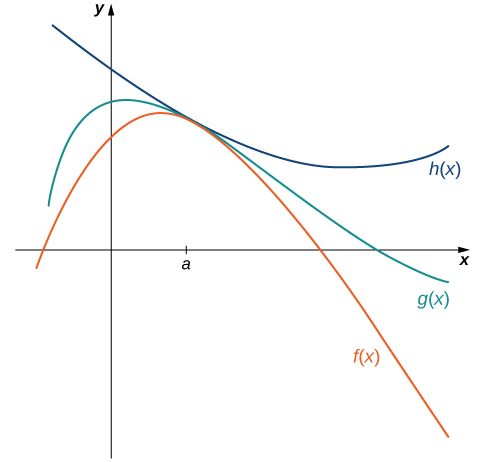
\includegraphics[scale=0.5]{img/CNX_Calc_Figure_02_03_005.jpeg}
}


\begin{example}
  Evaluate the limit
  \(\lim\limits_{x\to 0}\dfrac{\sin x}{x}\)
  
\begin{fullwidth}
  \begin{figure}[h!]
  \centering
  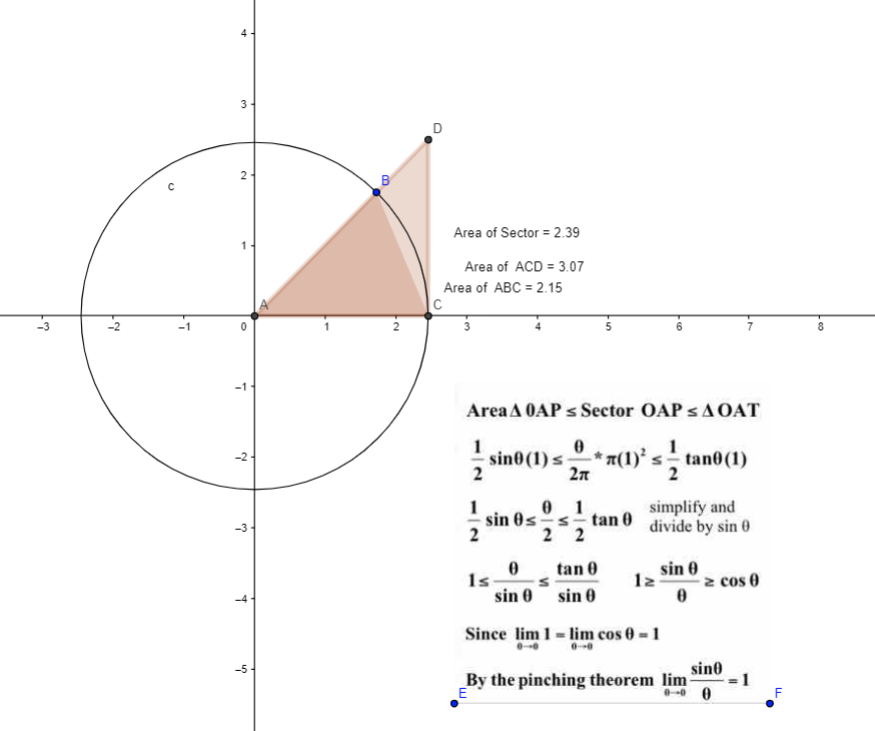
\includegraphics[width=0.8\linewidth]{img/image-20200830170927969.png}
  \end{figure}
\end{fullwidth}
\end{example}
\vspace*{6\baselineskip}

  
\begin{example}
Use the squeeze theorem to evaluate
\(\lim\limits_{x\to0}x^2\sin\dfrac{1}{x}\).

\href{https://www.geogebra.org/m/gb9uqf9u}{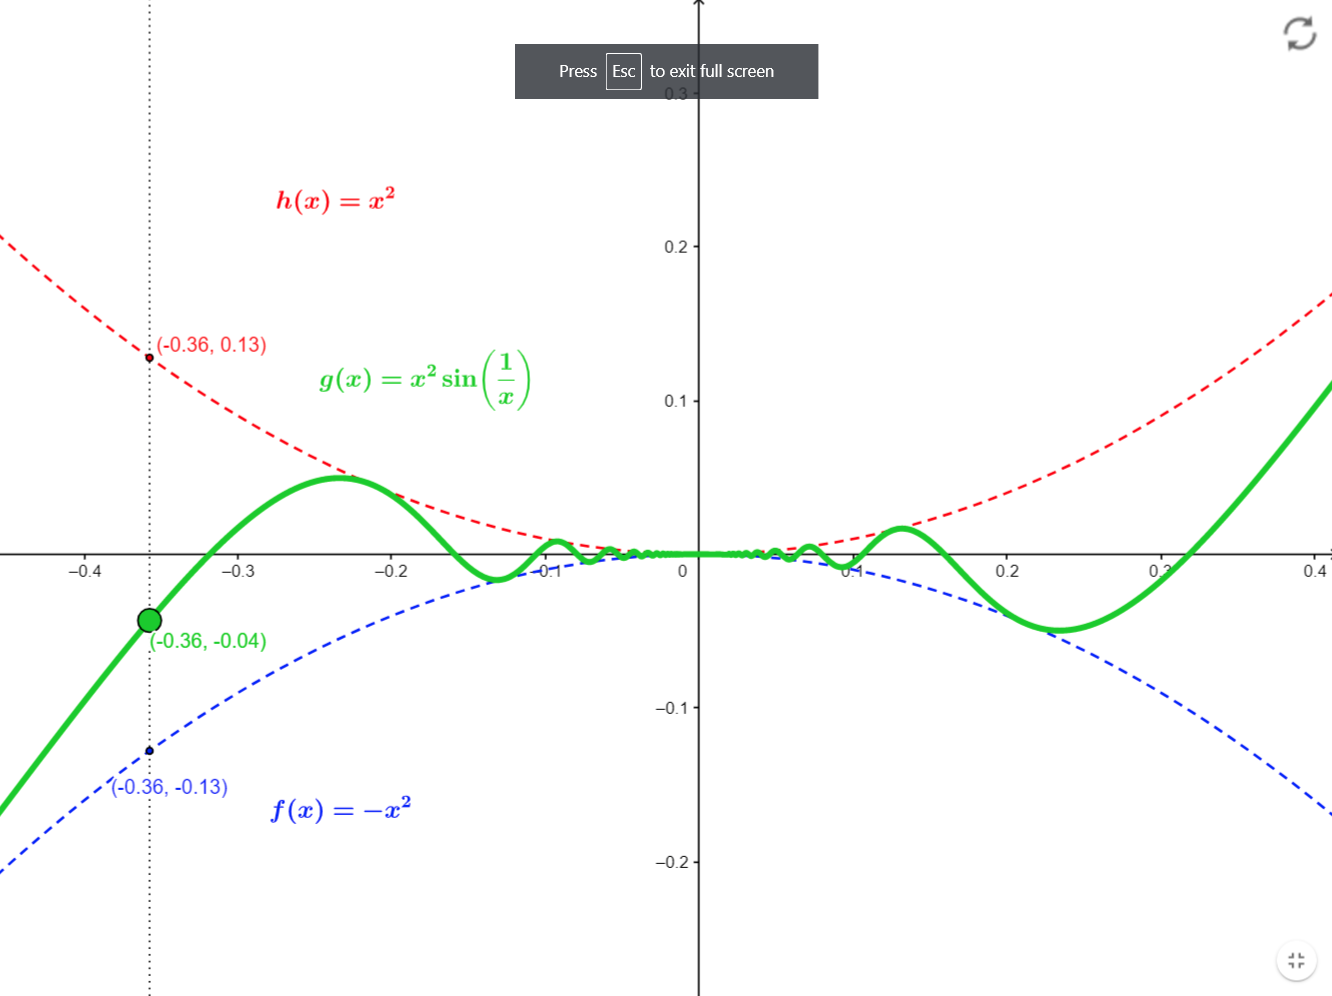
\includegraphics[width=0.9\textwidth]{img/image-20200830161044604.png}}
\end{example}
\vspace*{6\baselineskip}

\begin{example}
Suppose that
\(\lim\limits_{x\to a}\lvert f(x)-2\rvert =0\). Evaluate the limit
\(\lim\limits_{x\to a}f(x)\).
\end{example}
\vspace*{6\baselineskip}

\hypertarget{limits-of-indeterminate-forms}{%
\subsection{Limits of indeterminate
forms}\label{limits-of-indeterminate-forms}}

Some limits of indeterminate forms, such as \(\frac00\),
\(\frac{\infty}{\infty}\), \(0\cdot \infty\), and \(\infty-\infty\), can
be evaluated using algebraic methods. Here are some examples.

\begin{example}
Evaluate the limit
\(\lim\limits_{x\to 0}\dfrac{1-\cos x}{x}\)
\end{example}
\vspace*{6\baselineskip}

\begin{proposition}
  Let \(f\) be function defined near \(0\) and \(b\)
  be number. If \(\lim\limits_{x\to 0}\dfrac{f(x)}{x}=L\) and
  \(b \neq 0,\) then \(\lim\limits_{x \to 0}\dfrac{f(bx)}{x}=bL\).
\end{proposition}

\begin{example}
Evaluate the limit
\(\lim\limits_{\theta\to 0}\frac{\sin(3\theta)}{5\theta}\)
\end{example}
\vspace*{6\baselineskip}

\begin{example}
Evaluate
\(\lim\limits_{x\to 2}\left(\dfrac1{x^2-2x}-\dfrac{1}{2x-4}\right)\).
\end{example}
\vspace*{6\baselineskip}

\subsection{Apply limit laws to infinite
limits}

Limit laws mostly work for infinite limits. However, one should be very
careful when apply a limit laws with infinite limits.

\begin{example}
Evaluate \(\lim\limits_{x\to2^-}\dfrac{x-3}{x^2-2x}\).
\end{example}
\vspace*{6\baselineskip}

\subsection{Practice}

\begin{exercise}
  Evaluate
  \(\lim\limits_{x\to -1}\sqrt{\frac{8x^2-9x+10}{x^2+2}}\)
  \end{exercise}
  \vspace*{6\baselineskip}

\begin{exercise}
Evaluate \(\lim\limits_{x\to 3}\dfrac{x^2-9}{x-3}\).
\end{exercise}
\vspace*{6\baselineskip}

\begin{exercise}
Evaluate
\(\lim\limits_{x\to 49}\dfrac{\sqrt{x}-7}{x-49}\).
\end{exercise}
\vspace*{6\baselineskip}

\begin{exercise}
Evaluate
\(\lim\limits_{x\to 0}\lvert x\rvert \sin\left(\frac{1}{x}\right)\)
\end{exercise}
\vspace*{6\baselineskip}

\begin{exercise}
Evaluate
\(\lim\limits_{x\to 1}\left(\dfrac1{x^2-x}-\dfrac{1}{2x^2-3x+1}\right)\).
\end{exercise}
\vspace*{6\baselineskip}

\begin{exercise}
Evaluate the limit
\(\lim\limits_{t\to 0}\dfrac{\cos(3t)-1}{\sin t}\)
\end{exercise}
\vspace*{6\baselineskip}

\begin{exercise}
Evaluate
\(\lim\limits_{x\to 1}\dfrac{x+2}{(x-1)^2}\).
\end{exercise}
\vspace*{6\baselineskip}
